\chapter{Estrategia general del análisis de datos para la búsqueda de nueva física}
% \addcontentsline{toc}{chapter}{Estrategia general del análisis}
\chaptermark{Estrategia general del análisis de datos para la búsqueda de nueva física}



El análisis para el cual está orientada esta Tesis, consiste en la búsqueda de Supersimetría en eventos con un fotón aislado muy energético, jets y gran cantidad de energía faltante (\tosolve{cita fran y ultimos articulos}). La estrategia general de la búsqueda consiste en el conteo del número de eventos observado en exceso sobre el SM, en una cierta región del espacio de observables, rica en eventos de la señal considerada.


\section{Identificación de eventos de fondo}

Para un correcto procedimiento, es necesario conocer los procesos del SM que tengan un estado final equivalente a de la señal buscada. Estos eventos toman el rol de fondo en el contexto de un análisis de búsqueda de SUSY. Para este análisis, son procesos que tienen un fotón, jets y energía faltante en el estado final, y pueden dividirse en varias categorías. Por un lado, los procesos que dan lugar a eventos con un fotón y energía faltante
real, es decir, los que llamamos fondos irreducibles. Estos son:

\begin{itemize}

	\item $Z(\rightarrow \nu\nu)$ + $\gamma$

	\item $W (\rightarrow l\nu)$ + $\gamma$

	\item $t \overline{t}$ + $\gamma$

\end{itemize}

También es posible que, aunque el proceso no tenga fotones en el estado final, un electrón o un jet sean identificados como un fotón, dando lugar a un estado final idéntico al buscado. En esta categoría están:

\begin{itemize}

	\item $W (\rightarrow l\nu)$ + jets

	\item $Z (\rightarrow \nu\nu)$ + jets

	\item $t \overline{t}$

	\item $WW$, $ZZ$, $WZ$

\end{itemize}

Y por último, también puede haber procesos que a pesar de no generar energía faltante real, poseen lo que se denomina energía faltante instrumental, proveniente generalmente de la incorrecta reconstrucción de la energía de los jets. De esta manera, pueden dar lugar a eventos con el estado final de interés, los procesos QCD:

\begin{itemize}

	\item $\gamma$ + jets

	\item multijet, con alguno de los jets identificado como fotón

	\item $Z(\rightarrow ll)$ + jets, donde un leptón o un jet es identificado como un fotón

\end{itemize}



\section{Regiones de señal, control y validación}

Al estudiar fenómenos de nueva física es necesario definir una región en el espacio de observables, donde el modelo de señal predice un exceso significativo de eventos sobre el nivel de fondo. Esta región se llama región de señal (SR). El análisis consiste básicamente en estimar las contribuciones de los procesos del SM que contaminan esta región. Para esto existen dos técnicas principales: utilizar directamente simulaciones Monte Carlo, o utilizar métodos basados en los propios datos observados. En algunos casos se emplea un tercer método para estimar los fondos, que consiste en utilizar la estimación proveniente de las simulaciones MC, pero corregida a partir de los datos. Para esto se definen regiones de control (CR) en las cuales el fondo dominante pueda ser comparado y normalizado con los datos observados en esa misma región. 

Otra componente importante del análisis es la validación de los métodos utilizados para predecir los fondos. Con este objetivo se definen regiones de validación (VR) que se encuentren entre las CR y las SR en términos de los principales observables cinemáticos en los criterios de selección. El diseño de las VR comprende un compromiso entre minimizar la contaminación de la señal, y a su vez ser efectivas en la validación de la extrapolación entre CR y SR. Es importante que las CR, VR y SR sean estadísticamente independientes para poder combinar la pdf que modela cada región en una pdf conjunta. En la Figura \ref{regions} se puede ver como ejemplo, un esquema de las regiones descriptas anteriormente.

Durante todo el análisis se utiliza una estrategia denominada <<blinding>>. La misma consiste en realizar el análisis previo sin mirar la cantidad de eventos en la SR. De esta forma se evita un sesgo en la elección de las SR y por ende en la cantidad de eventos finales.

\begin{figure}
\centering
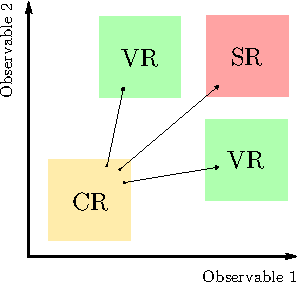
\includegraphics[width=0.40\textwidth]{regions}
\caption{Esquema del diseño de las regiones de señal (SR), control (CR) y validación (VR) en términos de dos observables arbitrarios.}
% \vspace{0.2cm}\footnotesize\textbf \sl{...}\vspace{0.2cm}
\label{regions}
\end{figure}

\section{Selección de eventos}

El análisis para el cual está orientada esta tesis \cite{Collaboration:2198651}, se basa en la utilización de dos regiones de señal, que son comparadas con las predicciones del SM. La primera de las regiones (SR$_{\text{L}}$), está optimizada para gluinos muy masivos y neutralinos con baja masa o intermedia. Se caracteriza por una alta multiplicidad de jets y actividad hadrónica, y baja energía faltante. La segunda región (SR$_{\text{H}}$) está orientada a escenarios donde la masa del gluino y el neutralino son más cercanas. Esto produce una baja multiplicidad de jets y actividad hadrónica, una producción de fotones de alto $p_{T}$ y una alta energía transversa faltante.

El modelo GGM predice gluinos muy masivos, por lo que es de esperar una elevada energía transversa total ($H_{T}$). Definiendo a $H_{T}$ como:

\begin{equation}
H_{T}=|p_{T}^{\gamma}|+\sum_{\text{jets}}|p_{T}^{\text{jet}}|
\end{equation} 
% comentario intencional para eliminar sangría
que es definitiva la suma escalar del momento transverso de todos los jets más la del fotón \textit{leading}. Para la selección de eventos de señal se utiliza una variable, $m_{\text{eff}}$, que es la suma escalar de $H_{T}$ y $\met$. En ambas regios se solicita que no se produzcan leptones y que se produzca al menos un fotón. Además, en la SR$_{L}$ más de 4 jets son requeridos, mientras que en la SR$_{H}$ más de dos.

En los eventos caracterizados por una elevada $\met$, el vector de energía transversa faltante tiende a estar alineado con el fotón o con alguno de los dos \textit{leading} jets. Para suprimir este fondo se utiliza una selección basada en la separación angular de estos objetos, $\Delta\phi$(jet, $\met$) y $\Delta\phi$($\gamma$, $\met$), para eventos con $\gamma$ + jets.

Finalmente se define una variable, $R_{T}^{4}$, definida como:

\begin{equation}
R_{T}^{4}=\frac{\sum_{i}^{4}p_{T}^{i}}{\sum_{\text{jets}}p_{T}^{j}}
\end{equation}
% comentario intencional para eliminar sangría
donde el numerador es una suma sobre los 4 jets con $p_{T}$ más alto, y el denominador es una suma sobre todos los jets. Las señales de SUSY consideradas en este análisis se caracterizan por tener varios jets con alto $p_{T}$, produciendo valores de $R_{T}^{4}$ menores a 1. Contrariamente, los fondos del SM no comparten esta característica, por lo que los valores de $R_{T}^{4}$ son cercanos a 1.

Los criterios de selección para ambas regiones de señal se resumen en la Tabla \ref{srs}.

\begin{table}
\centering
\caption{Criterios de selección para las SR$_{L}$ y SR$_{H}$. \tosolve{citar ICHEP}}
\begin{tabular}{ l | r | r }

	\hline

	& SR$_{L}$ & SR$_{H}$ \\

	\hline

	$N_{\text{fotones}}$ 	& $> 0$ 	& $> 0$ \\

	$N_{\text{leptones}}$ 	& $0$ 	& $0$ \\

	$N_{\text{jets}}$ 	& $>4$ 	& $>2$ \\

	$p_{T}^{\text{leading}\: \gamma}$ 	& $> 145 \egev$ 	& $> 400 \egev$ \\

	$\Delta\phi(jet,\: E_{T}^{\text{miss}})$ 	& $> 0.4$ 	& $> 0.4$ \\

	$\Delta\phi(\gamma$,\: $E_{T}^{\text{miss}})$ 	& $>0.4$ 	& $>0.4$ \\

	$\met$ 	& $>200\egev$ 	& $>400\egev$ \\

	$m_{\text{eff}}$ 	& $> 2000 \egev$ 	& $> 2400 \egev$ \\

	$R_{T}^{4}$ 	& $< 0.9$ 	& - \\

	\hline


\end{tabular}
\label{srs}
\end{table}

Para cada SR se asocian tres regiones de control, denominadas CRW, CRT y CRQ; utilizadas para la normalización de eventos de $W\gamma$, $\ttbar\gamma$ y QCD $\gamma + \text{jets}$, respectivamente. Las mismas variables que definen las SR son empleadas para establecer las CRs. Se agregan además otros requisitos para disminuir la contaminación o aumentar el numero de eventos de un cierto proceso; como por ejemplo colocar un máximo para la $E_{T}^{\text{miss}}$ o requerir la producción de b-jets. La tabla \ref{crs} muestra las selecciones utilizadas para definir las CRs.

\begin{table}
\centering
\caption{Criterios de selección para las CRs basadas a las SRs. Los valores son los mismos para SR$_{L}$ y SR$_{H}$.\tosolve{citar. estan bien los numeros? no hay MET y no importa el R4T}}
\begin{tabular}{ l | r r r }

	\hline

	 & CRQ & CRW & CRT \\

	 \hline

	$N_{\text{fotones}}$ 	& $\ge1$ & $\ge1$ & $\ge1$ \\

	$N_{\text{leptones}}$ 	& $0$ & $\ge1$ & $\ge1$ \\

	$N_{\text{jets}}>$ 		& $\ge3$ &	$\ge1$	& $\ge2$ \\

	$N_{\text{b-jets}}$ 	& - &	$0$	& $\ge2$ \\

	$p_{T}^{\text{leading}\: \gamma} [\egev]>$ 	& $145$ 	& $145$ 	& 	$145$ \\

	$\Delta\phi(jet,\: E_{T}^{\text{miss}})$ 	& $<0.4$ 	& $>0.4$ 	&  $>0.4$\\

	$\Delta\phi(\gamma$,\: $E_{T}^{\text{miss}})$	& $>0.4$ 	& - 	& -	\\

	$m_{\text{eff}} [\egev]>$ 	& $2000$ 	& $500$ 	& $500$	\\

	$R_{T}^{4}$ 	& - 	& - 	& -	\\

	\hline

\end{tabular}
\label{crs}
\end{table}


Junto con estas regiones se utilizan regiones de validación (VR), para verificar la estimación del fondo. Estas fueron diseñadas para ser similares a las SRs, pero con alguno de los criterios modificado o invertido, y de esta forma evitar que se contaminen con señal. Por ejemplo, una VR asociada a SR$_{H}$ se define con $m_{\text{eff}}>1000 \egev$ y con $125 \egev < E_{T}^{\text{miss}} < 175 \egev$. \tosolve{cual de todas las VR cito? hay muchas}